\chapter{MÉTODOS DE SOLUÇÕES}
%capítulo 4

Neste capítulo são apresentas as principais formas de soluções numéricas necessárias para o entendimento deste trabalho. Para tanto, a Seção \ref{Dinâmica} apresenta a Dinâmica dos Fluidos Computacional e suas diversas áreas de atuação. A seguir, é feita uma breve formulação do Método das Diferenças Finitas, Seção \ref{Dif_Fin}. Depois, é feita a análise de convergência, consistência e estabilidade, Seção \ref{Conver}, sendo que os problemas encontrados são corrigidos por meio do esquema de Lax-Friedrichs, Seção \ref{Lax_Fri}. Por fim, outras formas de tratar o domínio são apresentadas por meio do Método da Características, Seção \ref{Caracteristicas} e da Hidrodinâmica de Partículas Suavizadas, Seção \ref{Hidro_SPH}.

\section{DINÂMICA DOS FLUIDOS COMPUTACIONAL} \label{Dinâmica}

A solução de alguns problemas físicos podem se tornar uma tarefa árdua, senão impossível. Obter uma resposta algébrica para um conjunto de equações diferenciais parciais como as equações de Euler, exige muito tempo e, também, muitas simplificações podendo levar a resposta final distante da realidade. Para o caso das equações de Navier-Stokes, isso torna-se impossível.

A Dinâmica dos Fluidos mostrou bem a limitação do cálculo diferencial para prever fenômenos mais complexos, o que veio a prejudicar a hidrodinâmica por muitas décadas, conforme afirma \citeonline{Paiva2009}. 

A Dinâmica dos Fluidos Computacional (CFD), sigla em inglês de \textit{Computational Fluid Dynamics}, tem conseguido avanços consideráveis na modelagem e solução daquelas equações, pois alia o aprimoramento das técnicas e esquemas de soluções numéricas com a evolução da capacidade de processamento dos computadores. Isto faz com que fenômenos mais complexos sejam modelados com maior precisão e num espaço de tempo cada vez menor, bem como evita experimentos de altos custos ou impossíveis em laboratórios \cite{Crespo}.

\citeonline{Hirsch} esquematiza o desenvolvimento computacional de um experimento subdividindo-o em três etapas; Projeto Assistido por Computador (\textit{Computer-Assisted Design}-CAD), Engenharia Assistida por Computador (\textit{Computer-Assisted Engineering}-CAE) e Fabricação Assistida por Computador (\textit{Computer-Assisted Manufacturing}-CAM), onde cada uma destas etapas é formada por um conjunto de software e ferramentas computacionais. Dentro deste contexto, a CFD é classificada como um das formadoras da CAE, que também é composta pela Mecânica dos Sólidos Computacional (\textit{Computational Solid Mechanics}-CSM), Aeroacústica Computacional ( \textit{Computational Aero-Acoustics}-CAA) e Electromagnetismo Computacional (\textit{Computational electromagnetics}-CEM). Ao observar a posição central ocupada pela CAE e, dentro dela a CFD na Figura \ref{fig:esquema_CAE}, consegue-se compreender o que dizem \citeonline{Paiva2009} quando afirmam que pesquisadores em Dinâmicas dos Fluidos trabalham em institutos e departamentos de matemática, física e engenharia, o que torna esta área interdisciplinar.

\begin{figure}[H]
	\centering
	\includegraphics[scale=0.8]{figuras/esquema_CAE.jpg}
	\caption{\textsc{A estrutura de desenvolvimento de um protótipo virtual} }
	\vspace{-0.1cm}
	\legend{FONTE: Adaptado de \citeonline{Hirsch}}
	\label{fig:esquema_CAE}
\end{figure}
%\begin{figure}[h]
%\caption{A ESTRUTURA DE DESENVOLVIMENTO DE UM PROTÓTIPO VIRTUAL}
%\label{fig:esquema_CAE}
%\centering
%\includegraphics[scale=1]{esquema_CAE.jpg}
%\end{figure}

De uma forma geral, os métodos numéricos podem ser classificados em métodos eulerianos, que são aqueles que discretizam o domínio computacional por meio de um conjunto de células, comumente chamada de malha computacional ou \textit{grid}; métodos lagrangeanos, que são aqueles no qual utilizam um conjunto de partículas para discretizar o estado e a dinâmica de um sistema; os métodos híbridos, que são aqueles que combinam os métodos eulerianos e lagrangeanos, com o intuito de contornar as desvantagens que cada um deles apresentam, sendo normalmente usado em simulações que envolvem a interação fluido-estrutura. Este tipo de método numérico não será abordado neste trabalho, mas pode ser encontrado em trabalhos como \citeonline{Mao} ou \citeonline{Benson}. 

\section{MÉTODO DAS DIFERENÇAS FINITAS} \label{Dif_Fin}

Uma das ferramentas que compõem a CFD é a técnica euleriana das diferenças finitas, também chamada de Método das Diferenças Finitas (MDF), considerada a forma mais antiga de se obter a solução numérica das equações diferenciais, onde as primeiras aplicações foram atribuídas a Euler, em 1768 \cite{Hirsch}.

O MDF é baseado nas propriedades das expansões das séries de Taylor e nas aplicações diretas das definições de derivadas. Assim, considerando a definição da derivada da função $u$ em relação à $x$, tem-se:
\begin{equation} \label{derivu}
u' = \frac{ du}{ dx} = \lim_{ \Delta x \rightarrow 0} \frac{ u(x + \Delta x) - u(x)}{ \Delta x}.
\end{equation}

Se o limite for removido da igualdade acima, então resulta em uma diferença. Como $ \Delta x$ é pequeno, mas finito, obtêm-se uma aproximação para a função derivada $u$.

O fato de considerar $ \Delta x$ finito introduz um erro na solução da derivada, chamado de erro de truncamento e o tamanho deste erro pode ser obtido por meio da expansão por série de Taylor de $ u(x+ \Delta x)$ em torno de $x$, o que denomina-se de ordem de precisão da aproximação diferença \cite{Hirsch}. Então,  
\begin{equation} \label{Taylor}
u( x + \Delta x) = u(x) + \Delta x u'(x) + \frac{ \Delta x^2}{ 2!} u''(x) + \frac{ \Delta x^3}{ 3!} u'''(x) + \cdots 
\end{equation}
que pode ser escrita na forma
\begin{equation} \label{Taylortru}
\frac{ u( x + \Delta x) - u(x)}{ \Delta x} = u'(x) + \left[ \frac{ \Delta x}{2} u'' (x) + \frac{ \Delta x^{2}}{6} u''' (x) + \cdots \right]
\end{equation}
onde o termo entre colchetes é o erro de truncamento e, os demais termos considerados, confirmam que a igualdade (\ref{derivu}) é a definição para a derivada da função $u$ em relação à $x$.

Se na expressão (\ref{Taylortru}) for considerado o truncamento até o menor expoente em $ \Delta x$, ou seja,
\begin{equation} \label{Taylor_1}
\frac{ u( x + \Delta x) - u(x)}{ \Delta x} \approx u'(x) + \left[ \frac{ \Delta x}{2} u''(x) \right]
\end{equation}
a aproximação é dita de primeira ordem e escreve-se como
\begin{equation} \label{ordem_1}
\frac{ u( x + \Delta x) - u(x)}{ \Delta x} = u'(x) + O( \Delta x).
\end{equation}

É possível definir formas diferentes para aproximar a derivada e estas podem ter diferentes ordens de precisão. Contudo, a maneira como foram obtidas as formulações anteriores conduz à soluções contínuas para $u'(x)$, sendo que o objetivo é o cálculo de $u$ por meio de um conjunto discreto de pontos, ou seja, uma solução numérica. Desta forma, se for adotado um conjunto de pontos $x_i$, $i = 1, \ldots, N$, onde o domínio de interesse é subdividido em $N$ partes de tamanhos iguais $ \Delta x$ e $ u_i = ( i \Delta x)$, então a solução numérica pode ser encontrada, sem perda de generalidades, por meio de três caminhos da aproximação da derivada, que são
\begin{equation} \label{difav}
( u')_i = \frac{ u_{i+1} - u_i}{ \Delta x} + O( \Delta x),
\end{equation}
chamada de diferença avançada (\textit{forward difference})
\begin{equation} \label{difat}
( u')_i = \frac{ u_{i} - u_{i-1}}{ \Delta x} + O( \Delta x),
\end{equation}
chamada de diferença atrasada (\textit{backward difference}) e
\begin{equation} \label{difce}
( u')_i = \frac{ u_{i+1} - u_{i-1}}{2 \Delta x} + O( \Delta x^2),
\end{equation}
chamada de diferença central (\textit{central difference}).

Como pode ser observado, as diferenças (\ref{difav}) e (\ref{difat}) são de precisão de primeira ordem, enquanto que a diferença (\ref{difce}) é de precisão de segunda ordem. A interpretação geométrica destas diferenças pode ser observada na Figura \ref{fig:inter_geom}.

\begin{figure}[H]
	\centering
	\includegraphics[scale=1]{figuras/inter_geom.jpg}
	\caption{\textsc{Interpretação geométrica das fórmulas das diferenças para as derivadas de primeira ordem}}
	\vspace{-0.1cm}
	\legend{FONTE: adaptado de \citeonline{Hirsch}}
	\label{fig:inter_geom}
\end{figure}
%\begin{figure}[h]
%\caption{INTERPRETAÇÃO GEOMÉTRICA DAS FÓRMULAS DAS DIFERNÇAS PARA AS DERIVADAS DE PRIMEIRA ORDEM}
%\label{fig:inter_geom}
%\centering
%\includegraphics[scale=1]{inter_geom.jpg}
%\end{figure}

As fórmulas do Método das Diferenças Finitas unidimensional podem ser estendidas para o plano bidimensional. Ao observar a Figura \ref{fig:malha_2D} pode-se obter a malha retangular para o ponto $u_{ij} = u(x_i , y_j)$, sendo $ x_i = x_0 + i \Delta x$,  $ y_j = y_0 + j \Delta y$ e, então, para a diferença avançada na direção do eixo $x$,
\begin{equation} \label{avdir_x}
(u_x)_{ij} = \left( \frac{ \partial u}{ \partial x} \right)_{ij} = \frac{ u_{i+1,j} - u_{ij}}{ \Delta x} + O( \Delta x),
\end{equation}
ou, na direção do eixo $y$,
\begin{equation} \label{avdir_y}
(u_y)_{ij} = \left( \frac{ \partial u}{ \partial y} \right)_{ij} = \frac{ u_{i,j+1} - u_{ij}}{ \Delta y} + O( \Delta y) .
\end{equation}

Para a diferença atrasada na direção do eixo x,
\begin{equation} \label{atdir_x}
(u_x)_{ij} = \left( \frac{ \partial u}{ \partial x} \right)_{ij} = \frac{ u_{i,j} - u_{i-1,j}}{ \Delta x} + O( \Delta x)
\end{equation}
ou, na direção do eixo $y$,
\begin{equation} \label{atdir_y}
(u_y)_{ij} = \left( \frac{ \partial u}{ \partial y} \right)_{ij} = \frac{ u_{ij} - u_{i,j-1}}{ \Delta y} + O( \Delta y) .
\end{equation}

Para a diferença central na direção do eixo $x$,
\begin{equation} \label{cedir_x}
(u_x)_{ij} = \left( \frac{ \partial u}{ \partial x} \right)_{ij} = \frac{ u_{i+1,j} - u_{i-1,j}}{2 \Delta x} + O( \Delta x^2)
\end{equation}
ou, na direção do eixo $y$,
\begin{equation} \label{atdir_y}
(u_y)_{ij} = \left( \frac{ \partial u}{ \partial y} \right)_{ij} = \frac{ u_{i,j+1} - u_{i,j-1}}{2 \Delta y} + O( \Delta y^2) .
\end{equation}

\begin{figure}[H]
	\centering
	\includegraphics[scale=1]{figuras/malha_2D.jpg}
	\caption{\textsc{Malha cartesiana bidimensional}}
	\vspace{-0.1cm}
	\legend{FONTE: \citeonline{Hirsch}}
	\label{fig:malha_2D}
\end{figure}
%\begin{figure}[h]
%\caption{MALHA CARTESIANA BIDIMENSIONAL}
%\label{fig:malha_2D}
%\centering
%\includegraphics[scale=1]{malha_2D.jpg}
%\end{figure}

Outro caso a ser considerado para as diferenças é quando se deseja obter uma solução numérica para a função $u$ num tempo diferente daquele que está sendo trabalhado, ou seja, deseja-se conhecer a função para tempos diferentes, sendo que já se conhece a solução para o tempo atual $n$. Assim, discretizando o espaço e o tempo em intervalos constantes $ \Delta x$ e $ \Delta t$, sendo $x_i = i \Delta x$, $t^n = n \Delta t$ e $ u^{n}_{i} = u( i \Delta x, n \Delta t)$, pode-se obter duas formas de avaliar a solução. Para exemplificá-las, pode-se considerar a equação linear hiperbólica da advecção
\begin{equation}
\frac{ \partial u}{ \partial t} + a \frac{ \partial u}{ \partial x} = 0
\end{equation}
ou
\begin{equation} \label{advecção}
u_t + au_x = 0,
\end{equation}
sendo $a$ uma constante. Logo, adotando para a discretização no tempo a diferença avançada e para o espaço a diferença central, encontra-se
\begin{equation} \label{advnum}
\frac{ u^{n+1}_{i} - u^{n}_{i}}{ \Delta t} + \frac{a}{2 \Delta x} \left( u^{n}_{i+1} - u^{n}_{i-1} \right) = 0
\end{equation}
ou, explicitando o termo para o tempo $n+1$, 
\begin{equation} \label{explícito}
u^{n+1}_{i} =  u^{n}_{i} - \frac{a \Delta t}{2 \Delta x} \left( u^{n}_{i+1} - u^{n}_{i-1} \right) 
\end{equation} 
conhecido como Método das Diferenças Finitas Explícito (MDFE).

Da mesma forma, porém considerando o segundo termo da equação (\ref{advnum}) para o tempo $n+1$, tem-se
\begin{equation}
\frac{ u^{n+1}_{i} - u^{n}_{i}}{ \Delta t} + \frac{a}{2 \Delta x} \left( u^{n+1}_{i+1} - u^{n+1}_{i-1} \right) = 0,
\end{equation}
conhecido como o Método das Diferenças Finitas Implícito (MDFI).

De acordo com \citeonline{Sperandio}, a classificação das diferenças em explícitas ou implícitas está no fato de que se os valores de $u$, no tempo $n+1$, forem obtidos em função de todas as quantidades no tempo corrente $t=n$, então o método será explícito. No entanto, se $u$ for obtido por valores no tempo futuro, $t=n+1$, o método será implícito.

Uma ilustração da discretização no espaço e no tempo pode ser observada na Figura \ref{fig:espaço_tempo}.

\begin{figure}[H]
	\centering
	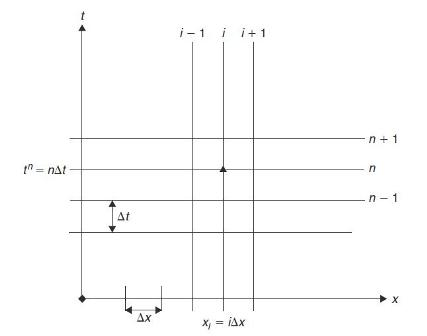
\includegraphics[scale=1]{figuras/espaco_tempo.jpg}
	\caption{\textsc{Discretização nos eixos espaço e tempo}}
	\vspace{-0.1cm}
	\legend{FONTE: \citeonline{Hirsch}}
	\label{fig:espaço_tempo}
\end{figure}

%\begin{figure}[h]
%\caption{DISCRETIZAÇÃO NOS EIXOS ESPAÇO E TEMPO}
%\label{fig:espaço_tempo}
%\centering
%\includegraphics[scale=1]{espaço_tempo.jpg}
%\end{figure} 

Conforme comentado em \citeonline{Press}, os métodos explícitos são de fácil implementação, pois a função é avaliada por meio de valores já conhecidos, o que os tornam muito econômicos em função do número de operações necessárias para avançar no tempo. Já para os esquemas implícitos, é necessário determinar três valores desconhecidos no tempo $n+1$, o que conduz a resolução de um sistema de equações tridiagonal, que pode ser linear ou não, dependendo da equação a ser resolvida. Para o caso de um sistema linear tridiagonal, o algoritmo de Thomas pode ser facilmente implementado. No entanto, para um sistema não linear o número de operações necessárias para o avanço no tempo pode ser muito maior.

De forma análoga ao que foi desenvolvido para as aproximações de segunda ordem no caso unidimensional, pode-se obter às aproximações de segunda ordem bidimensional, assunto amplamente discutido em literaturas como \citeonline{Tan} ou \citeonline{Leveque1992}.


\section{CONVERGÊNCIA, CONSISTÊNCIA E ESTABILIDADE} \label{Conver}

A falta de conhecimento das soluções exatas de certos problemas, nos remete à resolvê-los de forma aproximada por meio de um esquema ou método numérico. No entanto, faz-se necessário verificar até que ponto a forma numérica adotada é satisfatória para tal tarefa.

De acordo com \citeonline{Kundu}, a verificação da "qualidade" \ de um esquema numérico, seja ele implícito ou explícito, necessita de três conceitos: a convergência, a consistência e a estabilidade da solução numérica.

Segundo \citeonline{Crossley}, neste conjunto de conceitos ainda pode ser incluído a precisão, que define o quanto a solução aproximada está conseguindo representar da solução exata. Para tanto, se faz necessário o conhecimento de duas quantidades, que são: o erro local ou truncamento, que é a diferença entre a solução numérica em um dado ponto e a solução exata para este mesmo ponto, e o erro global, que reflete o erro total da solução numérica, o que quase sempre é impossível de se obter, já que a solução exata, no geral, é desconhecida.

Para \citeonline{Hirsch}, um esquema numérico é dito convergente quando a solução obtida tende para a solução exata no momento em que os passos, no tempo e no espaço, tendem para zero. Assim, o erro de truncamento pode ser definido como
\begin{equation}
\tilde{ \epsilon}^{n}_{i} = u^{n}_{i} - \tilde{ u} \left( i \Delta x , n \Delta t \right),
\end{equation}
onde $ \tilde{ u}(x,t)$ é a solução exata e, então, da condição de convergência, resulta que
\begin{equation}
\lim_{ \stackrel{ \Delta x \rightarrow 0}{ \Delta t \rightarrow 0} } | \tilde{ \epsilon}^{n}_{i} | = 0.
\end{equation}

\citeonline{Kundu} também afirmam que algumas medidas do erro podem ser estimadas por
\begin{equation}
\left\| e^{n}_{i} \right\| \leq k \Delta x^{a} \Delta t^{b} ,
\end{equation}
onde esta medida pode ser determinada como a raiz quadrada do erro médio, sendo $k$ uma constante que depende de $ \Delta x$ e $ \Delta t$, $a$ e $b$ são razões de convergência quando o erro se aproxima de zero.

Ao que foi visto acima, tudo leva a crer que um \textit{grid} pode ser reduzido indiscriminadamente e a convergência será sempre alcançada. No entanto, conforme afirma \citeonline{Crossley}, isto só será possível se o método for consistente, ou seja, ao ser reduzido o tamanho do passo no espaço e/ou no tempo a equação discretizada tender para a equação diferencial onde, neste caso, o método será dito como de uso prático.

Deve ser lembrado que, devido à aritmética finita dos computadores, pode haver um acúmulo no erro à medida que ocorre o avanço no tempo no processo de discretização. Se não houver um controle para este erro, a solução tenderá para o infinito e o método será dito instável. Portanto, um método será dito estável quando, ao avançar no tempo, mantiver o erro limitado. Isto é uma condição somente do método numérico utilizado e não envolve as condições da equação diferencial \cite{Hirsch}.

Muitos métodos numéricos tem o seu \textit{grid} limitado pelo número de Courant-Friedrichs-Lewy ($Co$),
\begin{equation} \label{CFL}
Co \leq 1
\end{equation}
o que indica que a partícula de um fluido não pode percorrer mais do que um \textit{grid} espacial em um passo de tempo.

Dentre os conceitos analisados, a estabilidade é decisiva para a viabilidade de uma aproximação numérica, devido ser uma condição necessária (em vez de suficiente) para se ter a precisão. A relação entre consistência, estabilidade e convergência é conhecida como o Teorema da Equivalência de Lax \cite{Hirsch}.
\begin{theorem}[Teorema de Lax]
	Dada uma equação diferencial parcial com condições iniciais e de contorno, bem postas, e um esquema de discretização que satisfaz à condição de consistência, então a estabilidade é uma condição necessária e suficiente para a convergência.
\end{theorem}

Pode-se adotar três procedimentos para a análise de estabilidade, que são: a estabilidade eurística, a estabilidade de Von Neumann e a estabilidade matricial. Destes, o mais utilizado, segundo \citeonline{Sperandio}, é a análise de Von Neumann que, basicamente, representa o erro numérico via uma decomposição harmônica de Fourier, ou seja,
\begin{equation} \label{Von_Neumann}
u^{n}_{j} = \xi ^{n} e^{ ikj \Delta x}, 
\end{equation}
onde $k$ é um número de onda espacial real e $ \xi = \xi (k)$ é um número complexo que depende de $k$, chamado de fator de amplificação. Em seguida, a decomposição harmônica é substituída na equação discretizada e, então, é feita a análise do crescimento do erro, determinando assim se o método é condicionalmente estável ou incondicionalmente estável. Mais detalhes do assunto podem ser vistos em \cite{Hirsch}, \cite{Kundu}, \cite{Sperandio} ou \cite{Batchelor}.

%-------------------------------------------------------------------------------------------------------------------------------------------------------
\section{O ESQUEMA DE LAX-FRIEDRICHS} \label{Lax_Fri}

Como mostrado anteriormente, a equação linear hiperbólica da advecção, equação (\ref{advecção}), foi discretizada por meio do MDFE, equação (\ref{explícito}). No entanto, a forma como foi construída esta discretização gera instabilidade que, segundo o Teorema de Lax, não será convergente. Nota-se isso por meio da análise de Von Neumann que, ao substituir o fator de amplificação (\ref{Von_Neumann}) na equação (\ref{explícito}), resulta
\begin{equation} \label{instabi}
\xi (k) = 1-i(Co)sen(k \Delta x),
\end{equation}
onde $ Co = {a \Delta t}/{ \Delta x} \leq 1$, é o número de Courant-Friedrichs-Lewy, desigualdade (\ref{CFL}), e $i$ é um número imaginário.

De acordo com \citeonline{Press}, como 
\begin{equation}
| \xi (k)| = |1-i(Co)sen(k \Delta x)| >1,
\end{equation}
para todo $k$, então o método é incondicionalmente instável. A Figura \ref{fig:Dias_A} mostra as instabilidades geradas para alguns intervalos de tempo.

\begin{figure}[H]
	\centering
	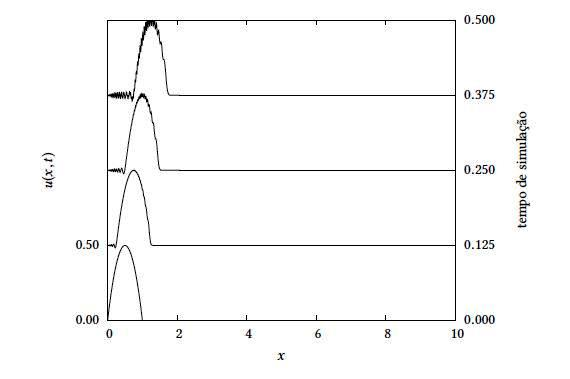
\includegraphics[scale=1]{figuras/Dias_A.jpg}
	\caption{\textsc{Solução numérica da equação da advecção por meio do MDFE}}
	\vspace{-0.1cm}
	\legend{FONTE: Autoria própria}
	\label{fig:Dias_A}
\end{figure}

Para tentar solucionar o problema da instabilidade o esquema de Lax-Friedrichs substitui o termo $u^{n}_{i}$, na equação (\ref{explícito}), por um termo médio, ou seja, 
\begin{equation} \label{ELF}
u^{n}_{i} = \frac{1}{2} \left( u^{n}_{i+1} + u^{n}_{i-1} \right).
\end{equation}
Dessa forma, a equação (\ref{explícito}) passa a ser escrita como
\begin{equation} \label{esq_Lax}
u^{n+1}_{i} =  \frac{1}{2} \left[ \left( u^{n}_{i+1} + u^{n}_{i-1} \right)  - (Co) \left( u^{n}_{i+1} - u^{n}_{i-1} \right) \right]. 
\end{equation} 

Ao fazer a análise de estabilidade de Von Neumann na equação (\ref{esq_Lax}) encontra-se que
\begin{equation} \label{instabi_Lax}
\xi (k) = cos(k \Delta x)-i(Co)sen(k \Delta x).
\end{equation}

Se $ \xi (k)$ na equação (\ref{instabi_Lax}), que é um número complexo, for maior do que $1$, então o esquema (\ref{esq_Lax}) será instável, mas se for considerado que $ | \xi (k)|^{2} \leq 1$ o esquema (\ref{esq_Lax}) será estável, o que só será possível se $Co \leq 1$, que é o critério de Courant-Friedrichs-Lewy.

Segundo \citeonline{Press}, o que ocorre no esquema de Lax-Friedrichs é a inclusão de um termo difusivo, ou seja, o esquema de Lax-Friedrichs é dito ter uma dissipação numérica ou viscosidade numérica. Isto pode ser observado na Figura \ref{fig:Dias_B}, onde não ocorre mais as soluções espúrias que estavam ocorrendo na Figura \ref{fig:Dias_A}, mostrando que o esquema (\ref{esq_Lax}) é estável. No entanto, a solução é "amortecida" \ pela difusão numérica, o que pode prejudicar a resposta do ponto de vista físico do problema. Existem outras forma de contornar o problema da instabilidade encontrada pelo MDFE, como o método de Lax-Wendroff ou mesmo o esquema Upwind, mas não serão abordados neste trabalho. Tais métodos podem ser encontrados em literaturas como \citeonline{Press}, \citeonline{Hirsch}, \citeonline{Kundu}, \citeonline{Sperandio} ou \citeonline{Batchelor}.

\begin{figure}[H]
	\centering
	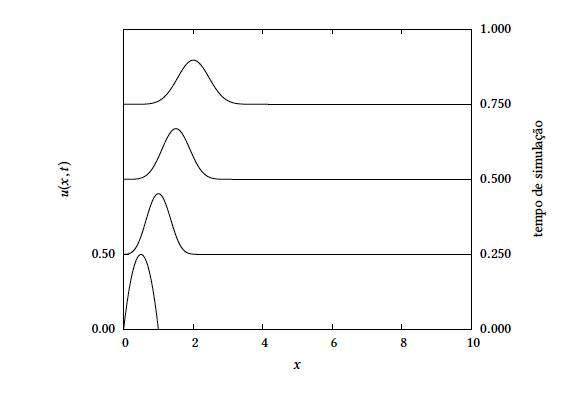
\includegraphics[scale=1]{figuras/Dias_B.jpg}
	\caption{\textsc{Solução numérica da equação da advecção por meio do esquema de Lax-Friedrichs}}
	\vspace{-0.1cm}
	\legend{FONTE: Autoria própria}
	\label{fig:Dias_B}
\end{figure}
%-------------------------------------------------------------------------------------------------------------------------------------------------------

\section{MÉTODO DAS CARACTERÍSTICAS} \label{Caracteristicas}

Define-se como "características" \ linhas no plano espaço-tempo ao longo das quais certas propriedades das Equações Diferenciais Parciais (EDPs) se propagam e o método pode ser considerado como uma forma analítica de obter suas soluções \cite{Cunge}.

Utilizando como exemplo a EDP de primeira ordem
\begin{equation}\label{exempcarac}
u_t +a(x,t)u_x=0,
\end{equation}
com condição inicial $u(x,0)=u_0$. Pode-se definir, pela regra da cadeia \cite{Leithold}, que
\begin{equation*}
\frac{du}{dt} = u_t + \frac{dx}{dt}u_x,
\end{equation*}
ou seja, 
\begin{equation} \label{uisolado}
u_t = \frac{du}{dt} - \frac{dx}{dt}u_x.
\end{equation}

Substituindo a equação (\ref{uisolado}) na equação (\ref{exempcarac}) defini-se que
\begin{equation} \label{CaracIsol}
\frac{du}{dt} + \left( a(x,t) -\frac{dx}{dt} \right)u_x = 0.
\end{equation}

Observando a equação (\ref{CaracIsol}) percebe-se que ${du}/{dt} = 0$ em toda linha definida por ${dx}/{dt} = a(x,t)$. Isso implica que a solução $u$ é constante ao logo daquela linha, conhecida como linha característica.

Se for possível definir um conjunto de linhas características, então será possível conhecer a solução para todos os tempos, sendo necessário para isso apenas as condições iniciais e as condições do contorno do problema, desde que as linhas não se interceptem. Assim, pode-se obter a solução do problema, equação (\ref{exempcarac}), por
\begin{equation}
u(x,t) = u \left( x - \int\limits_{0}^{t} a(x,t) dt , 0 \right).
\end{equation}  

Considerando o domínio do problema uma região finita, conforme a Figura \ref{fig:dominiofinito}, para obter uma solução é necessário especificar os valores ao longo de alguma fronteira que contém as linhas características. Por exemplo, se for especificado o valor ao longo da linha $x=x_1$, não será necessário especificar os valores das demais linhas, pois as linhas características, dentro da região finita, já serão conhecidas.

\begin{figure}[H]
\centering
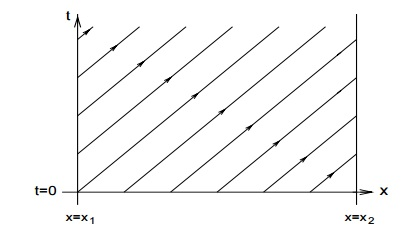
\includegraphics[scale=1.2]{figuras/Caracteristica.jpg}
\caption{\textsc{Linhas características sobre um domínio finito}}
\vspace{-0.1cm}
\legend{FONTE: \citeonline{Crossley}}
\label{fig:dominiofinito}
\end{figure}


Se for considerado o caso em que
\begin{equation}
u_t + a(u)u_x = 0,
\end{equation}
onde $ f'(u) = a(u)$, então
\begin{equation}
u_t + f(u)_x = 0
\end{equation}
será uma lei de conservação escalar, sendo a característica dada por
\begin{equation}
\frac{dx}{dt} = a(u).
\end{equation}

Definido $u$ como constante ao longo da linha característica acima, $a$ também será constante, sendo que todas as características serão linhas retas e, pela teoria das Equações Diferenciais Ordinárias (EDOs) \cite{kreyszig}, será possível mostrar que, para $u$ contínuo, as linhas características não irão se interceptar. No entanto, as EDPs hiperbólicas admitem soluções descontínuas e, para uma lei de conservação hiperbólica não linear, as linhas características irão se interceptar formando descontinuidades ou choques, como pode ser observado nas interpretações geométricas construídas no trabalho de \citeonline{Adilandri}.

%-------------------------------------------------------------------------------------------------------------------------------------------------------
\section{HIDRODINÂMICA DE PARTÍCULAS SUAVIZADAS} \label{Hidro_SPH}

Além do MDF, outra ferramenta da CFD são os métodos lagrangeanos sem malhas baseados em partículas (\textit{meshfree methods}). Estes tipos de métodos vêm ganhando espaço na modelagem computacional, principalmente com a melhora na capacidade de processamento dos computadores e com a crescente programação direta em placas gráficas, como pode ser visto no trabalho de \citeonline{Harada}.

De acordo com \citeonline{Queiroz}, estes métodos possuem a vantagem de se adaptarem a grandes deformações, de suportarem mudanças topológicas e de lidarem de forma "robusta" \ com os refinamentos adaptativos para o controle da precisão dos resultados. Em contrapartida, possuem como principal desvantagem o custo computacional na busca por partículas vizinhas, já que necessitam das informações particulares de cada uma delas para avançar no tempo.

Dentre os métodos sem malhas existentes, o Método das Partículas Suavizadas ( \textit{Smoothed Particle Hydrodynamics}-SPH), se destaca nas simulações de escoamentos de fluidos, pois permite estas realizações em tempo linear, o que é desejável para aplicações em tempo real (\citeonline{Muller}, \textit{apud} \citeonline{Queiroz}).

O SPH surgiu para modelar fenômenos astrofísicos nos trabalhos desenvolvidos por \citeonline{Lucy} e \citeonline{Gingold}. A ideia básica deste método consiste em substituir o domínio físico por um domínio discretizado por meio de partículas (núcleos), onde cada um destes núcleos possui propriedades como pressão, densidade, velocidade, etc. Para cada ponto do domínio, a função ou uma de suas derivadas é aproximada por uma média ponderada das contribuições de todas as partículas que estão próximas deste ponto, ou seja, é feita uma convolução, conforme comentado em \citeonline{Paiva2009}. Assim, dada uma função $f$ definida sobre um volume $\Omega$, tem-se:
\begin{equation} \label{integral}
f(\textbf{r}) = \int_{\Omega} f(\textbf{r'})\delta(\textbf{r}-\textbf{r'})dr',
\end{equation}
onde $\delta$ é a função Delta de Dirac, $\textbf{r}$ e $\textbf{r'}$ são variáveis no domínio de $\Omega$.

Da definição da função Delta de Dirac, \cite{Queiroz}, tem-se
\begin{equation}
\delta = \left\{
\begin{array}{rcl}
1 & se & \textbf{r} = \textbf{r'}\\
0 & se & \textbf{r} \neq \textbf{r'}
\end{array} \right.
\end{equation}
e
\begin{equation}
\int_{\Omega} \delta(\textbf{r}-\textbf{r'})dr =1.
\end{equation}

Apesar do uso da função Delta de Dirac na equação (\ref{integral}), isto é apenas uma função generalizada, pois nenhuma função pode ter as mesmas propriedades que ela. Desta forma, pode-se afirmar que a equação (\ref{integral}) não é compatível e deve-se substituir a função Delta de Dirac por uma função que se comporte como ela. Tal função é a função núcleo suavizado (\textit{Smooth Kernel}) $W(\textbf{r},h)$, onde $h$ é o comprimento de suavização (\textit{Smooth Lenght}), devendo satisfazer as seguintes propriedades:
\begin{enumerate}
	\item[1)] $W$ deve se aproximar do comportamento da função $\delta$ quando $h$ tende para zero, o que garante a consistência da equação (\ref{integral})
	\begin{equation}
	\lim\limits_{h \rightarrow 0} W(\textbf{r},h) = \delta(\textbf{r}).
	\end{equation}
	
	\item[2)] Assim como a função $\delta$, $W$ deve ser normalizada
	\begin{equation}
	\int_{\Omega} W(\textbf{r},h) dr' = 1.
	\end{equation}
	
	\item[3)] A função núcleo deve possuir um suporte compacto, ou seja, deve ser nula sempre que o comprimento for maior do que $kh$, sendo $k$ uma constante relacionada com o comprimento de suavização
	\begin{equation}
	W(\textbf{r},h) = 0 ; |\textbf{r} - \textbf{r'}| > kh.
	\end{equation}
	
	\citeonline{Paiva2009} destaca ainda que a função núcleo deve satisfazer mais três propriedades, que são:
	\item[4)] O núcleo deve ser sempre positivo no suporte compacto, pois se for negativo pode afetar a densidade
	\begin{equation}
	W(\textbf{r},h) \geq 0.
	\end{equation}
	
	\item[5)] O núcleo deve ser sempre decrescente, ou seja, as partículas mais distantes do núcleo central tem menor influência sobre ele
	\begin{equation}
	W(\textbf{x},h) < W(\textbf{r},h)  \\ se \\ \parallel \textbf{x} \parallel > \parallel \textbf{r} \parallel.
	\end{equation}        
	
	\item[6)] O núcleo deve ser simétrico, o que pode ser mostrado por meio da expansão de $W(\textbf{r} - \textbf{r'},h)$ por série de Taylor \cite{Monaghan1992}
	\begin{equation}
	W(\textbf{r} - \textbf{r'},h) = W(\textbf{r'} - \textbf{r},h).
	\end{equation}
\end{enumerate}

Satisfeitas as propriedades anteriores, substituindo o volume infinitesimal $dr'$ por um volume finito $\Delta V$, representado por partículas vizinhas, e relacionado este volume com a massa $m$ de uma das partícula por meio da expressão $m= \Delta V \cdot \rho$, então a equação (\ref{integral}) pode ser discretizada por
\begin{equation} \label{aprox_SPH}
f(\textbf{r}) \approx \sum\limits_{i} \frac{m_{i}}{\rho_{i}} f(\textbf{r}_{i}) W(\textbf{r} - \textbf{r}_{i},h),
\end{equation} 
onde $i$ é uma distância sobre todas as partículas próximas ao núcleo suavizado. As Figuras \ref{fig:nucleo_B} e \ref{fig:nucleo_A} mostram esquemas representativos da função núcleo, sendo que na Figura \ref{fig:nucleo_A} tem-se ainda a representatividade da influência que as partículas vizinhas exercem sobre o núcleo.

\begin{figure}[H]
	\centering
	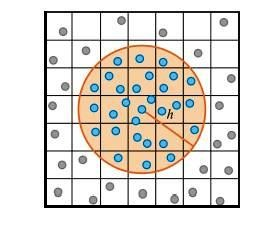
\includegraphics[scale=1]{figuras/nucleo_B.jpg}
	\caption{\textsc{Representação do núcleo no suporte compacto}}
	\vspace{-0.1cm}
	\legend{FONTE: \citeonline{Bruno}}
	\label{fig:nucleo_B}
\end{figure}

\begin{figure}[H]
	\centering
	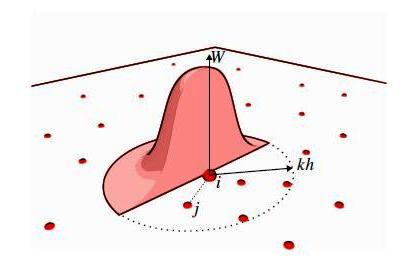
\includegraphics[scale=1]{figuras/nucleo_A.jpg}
	\caption{\textsc{Representação do núcleo no suporte compacto sob a influência das partículas dentro do raio $kh$}}
	\vspace{-0.1cm}
	\legend{FONTE: \citeonline{Queiroz}}
	\label{fig:nucleo_A}
\end{figure}       

A forma como a função $f$ foi discretizada na equação (\ref{aprox_SPH}) para uma posição $\textbf{r}$, num domínio computacional $\Omega$, é a base de todo o formalismo do SPH.

Como visto nas propriedades, a escolha do núcleo é importante para a correta discretização da função $f$ e diferentes funções podem ser utilizadas para cumprir tal tarefa. \citeonline{Gingold} propuseram, como função núcleo, a função gaussiana
\begin{equation}
W(\textbf{r} - \textbf{r'},h) = \frac{1}{h^{3} \pi^{3/2}} e^{-x^{2}},
\end{equation}
sendo, $x = {| \textbf{r} - \textbf{r'}|}/{h}$. No entanto, esta função não possui suporte compacto, mas aproxima-se rapidamente de zero, sem nunca atingi-lo, quando as distâncias entre duas partículas aumenta. Assim, ocorrerá a inclusão de muitas partículas na vizinhança, conforme a Figura \ref{fig:nucleo_B}, o que terá um custo computacional alto demais.

Outro tipo de função amplamente utilizada são as funções Splines. No trabalho de \citeonline{Monaghan1985} foi proposto o uso da função spline cúbica  
\begin{equation}
W(\textbf{r} - \textbf{r'},h) = \frac{1}{\pi h^{3}} \left\{
\begin{array}{rcl}
1 - \frac{3}{2} x^{2} + \frac{3}{4} x^{3} & se & 0 \leq x < 1 \\
\frac{1}{4}(2-x)^{3} & se & 1 \leq x < 2 \\
0 & se & x \geq 2,  
\end{array} \right.
\end{equation}
onde somente partículas que distam $2h$ do centro contribuem para a suavização do núcleo. Splines de maior grau também são utilizadas para aproximação do núcleo, bem como outras variações, como aquelas propostas no trabalho de \citeonline{Lucy}. No entanto, todas apresentam problemas em satisfazer as propriedades necessárias. A Figura \ref{fig:nucleos} mostra o comportamento de três núcleos, sendo que o núcleo spline cúbico é o que melhor se compara com o gaussiano, por isso é o mais utilizado. Já a Figura \ref{fig:pricePDF4} mostra o comportamento de outras funções spline representando o núcleo. Mais detalhes sobre as funções núcleo podem ser encontrados na bibliografia como \citeonline{Paiva2009} ou  \citeonline{Violeau}.

\begin{figure}[H]
	\centering
	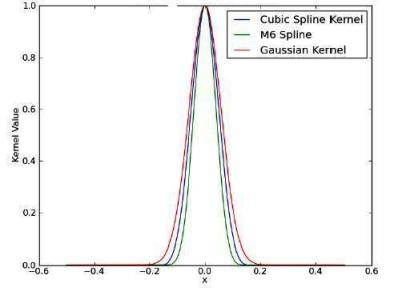
\includegraphics[scale=1]{figuras/nucleos.jpg}
	\caption{\textsc{Comparação das funções splines de terceiro e quinto graus com a função gaussiana}}
	\vspace{-0.1cm}
	\legend{FONTE: \citeonline{CodigoPySPH}}
	\label{fig:nucleos}
\end{figure} 

\begin{figure}[H]
	\centering
	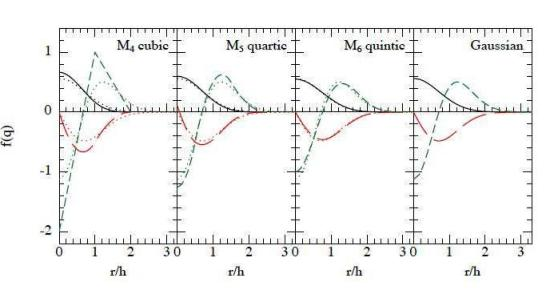
\includegraphics[scale=1]{figuras/pricePDF4.jpg}
	\caption{\textsc{Comparação das funções splines de terceiro, quarto e quinto graus e suas derivadas, primeira e segunda, linhas pontilhadas longas e curtas, respectivamente, com a função gaussiana}}
	\vspace{-0.1cm}
	\legend{FONTE: \citeonline{Price}}
	\label{fig:pricePDF4}
\end{figure} 

Uma vez determinado o núcleo, a modelagem por meio do SPH necessita das derivadas de alguns campos, como os vetoriais e escalares. Assim, considerando a equação (\ref{integral}) como um campo escalar, seu gradiente pode ser avaliado por
\begin{equation}
\nabla f(\textbf{r}) = \frac{\partial}{\partial \textbf{r}} \int\limits_{\Omega} f({\textbf{r'}) \delta (\textbf{r} - \textbf{r'})}dr',
\end{equation}  
cuja aproximação, por intermédio de (\ref{aprox_SPH}) , resulta em
\begin{equation} \label{esc_SPH}
\nabla f(\textbf{r}) \approx \sum\limits_{i} \frac{m_{i}}{\rho_{i}} f(\textbf{r}_{i}) \nabla W(\textbf{r} - \textbf{r}_{i},h).
\end{equation}

Se a equação (\ref{integral}) for considerada como um campo vetorial, $\vec{F(\textbf{r})}$, então
\begin{equation}
\vec{F(\textbf{r})} = \int\limits_{V} \vec{F(\textbf{r'})} \delta (\textbf{r} - \textbf{r'})dr'.
\end{equation} 
Assim, calculando o seu divergente em relação à $\textbf{r}$, a aproximação integral torna-se
\begin{equation} \label{div_SPH}
\nabla \cdot \vec{F(\textbf{r})} \approx \sum\limits_{i} \frac{m_{i}}{\rho_{i}} \vec{F(\textbf{r}_{i})}  \cdot \nabla W(\textbf{r} - \textbf{r}_{i},h). 
\end{equation}

De forma análoga, pode-se determinar o rotacional do campo vetorial $\vec{F(\textbf{r})}$, ou seja, $\nabla \times \vec{F(\textbf{r})}$ sendo aproximado por
\begin{equation} \label{rot_SPH}
\nabla \times \vec{F(\textbf{r})} \approx \sum\limits_{i} \frac{m_{i}}{\rho_{i}} \vec{F(\textbf{r}_{i})}  \times \nabla W(\textbf{r} - \textbf{r}_{i},h).
\end{equation}

Conforme comentado em \citeonline{Paiva2009}, alguns destes operadores são imprecisos e podem não obedecer as propriedades de conservação quando utilizados na simulação do escoamento de fluidos. Deste forma, existem variações das aproximações dos campos escalares e vetoriais. Os erros destas aproximações, bem como outras formas de aproximar os gradientes e divergentes daqueles campos, podem ser encontrados em \citeonline{Monaghan1992}.

A representação do escoamento de um fluido, por meio da discretização do SPH, inicia-se com a representação da densidade de uma partícula específica $\rho_{j}$, diretamente da aproximação (\ref{aprox_SPH}). Assim, pode-se considerar que
\begin{equation}
\rho_{j} = \sum\limits_{i} m_{i} W(\textbf{r}_{j} - \textbf{r}_{i},h)
\end{equation}
ou, de forma simplificada,
\begin{equation} \label{Densi_PSH}
\rho_{j} = \sum\limits_{i} m_{i} W_{ji}.
\end{equation} 

Novamente por \citeonline{Paiva2009}, o cálculo da densidade usando a equação aproximada (\ref{Densi_PSH}) exige um esforço adicional na implementação numérica, pois a densidade deve ser calculada em primeiro lugar para todas as partículas, antes dos demais parâmetros. Uma alternativa é a substituição de uma das formas dos divergentes, como a equação (\ref{div_SPH}), diretamente na equação da continuidade (\ref{eq_massa_2}), o que resulta 
\begin{equation} \label{Cont_SPH}
\frac{d \rho_{j}}{dt} = -\rho_{j} \sum\limits_{i} \frac{m_{i}}{\rho_{i}} (\textbf{v}_{i} - \textbf{v}_{j}) \cdot \nabla_{j}W_{ji},
\end{equation}
que é a equação da Continuidade na formulação SPH, onde $\textbf{v}_{i} = {d \textbf{r}_{i}}/{dt}$ e $\textbf{v}_{j} = {d \textbf{r}_{j}}/{dt}$.

De acordo com \citeonline{Cossins}, como a discretização é feita sob uma dada partícula em um meio contínuo, pode ser considerada a derivada total para determinar a equação da Continuidade, conforme mostrado na equação (\ref{Cont_SPH}). Assim, também para a equação de Conservação do Movimento (\ref{eq_movimento_final}), a aproximação SPH é dada por
\begin{equation} \label{Mov_SPH}
\frac{d \textbf{v}_j}{dt} = -\sum\limits_{i}m_{i} \left( \frac{P_j}{\rho^{2}_{j}} + \frac{P_i}{\rho^{2}_{i}} \right) \nabla_{j}W_{ji}.
\end{equation}

Para a equação da Energia Total (\ref{Energi_T}),  a aproximação SPH é dada por
\begin{equation} \label{energ_SPH}
E = \sum\limits_{i} m_{i} \left( \frac{1}{2} \textbf{v}_{i} \cdot \textbf{v}_{i} + e_{i} \right),
\end{equation}
cuja derivada no tempo resulta em
\begin{equation}
\frac{dE}{dt} = \sum\limits_{i} \sum\limits_{j}  m_{i}  m_{j} \left( \frac{P_j}{\rho^{2}_{j}} \textbf{v}_{i} +  \frac{P_i}{\rho^{2}_{i}} \textbf{v}_{j} \right) \cdot \nabla_{j}W_{ji} 
\end{equation}
que, novamente por \citeonline{Cossins}, é conservativa.

A implementação computacional usando o método SPH deve seguir uma sequência lógica de operações, já que cada partícula transporta consigo propriedades físicas inerentes ao fluido que está sendo modelado e, a cada passo de tempo, sofre a influência das demais partículas que estão no seu suporte compacto. Além do mais, com o avanço no tempo, as posições não são preservadas, fazendo com que a simulação total sofra constantes atualizações. Desta forma, se o algoritmo não for eficiente, capaz de "prever" \ estas particularidades do método, acabará comprometendo a simulação.

No trabalho de \citeonline{Paiva2009} é apresentado um visão simplificada da implementação por meio do SPH, conforme pode ser observado na Figura \ref{fig:visao}. Deste esquema simplificado destacam-se dois pontos principais que podem afetar a simulação, que são: a busca por partículas vizinhas e as condições de fronteira.
\begin{figure}[H]
	\centering
	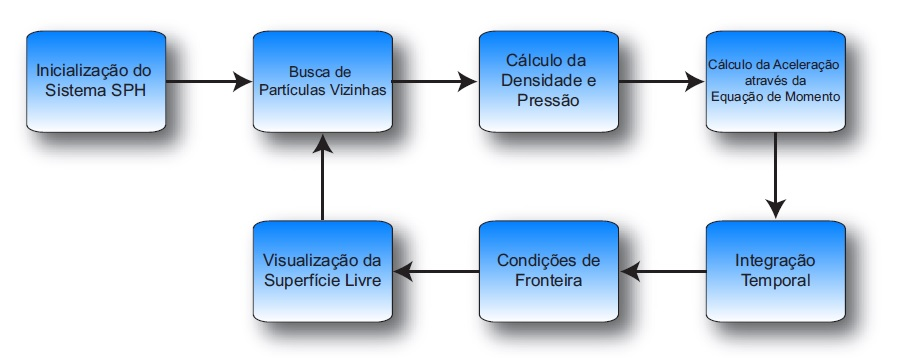
\includegraphics[scale=0.9]{figuras/visao.jpg}
	\caption{\textsc{Visão simplificada da implementação computacional usando o SPH}}
	\vspace{-0.1cm}
	\legend{FONTE: \citeonline{Paiva2009}}
	\label{fig:visao}
\end{figure}

No SPH as partículas estão sempre mudando de posição, então é necessário uma atualização constante dos vizinhos de cada núcleo. Um dos métodos utilizados para realizar esta tarefa é o da Força Bruta, que verifica quais as partículas estão a uma distância inferior a $kh$ de um determinado núcleo e as considera no suporte compacto. É um método simples, mas pode ser muito custoso, pois a medida que o número $n$ de partículas aumenta exige um esforço computacional maior, já que eleva o tempo computacional à ordem $O(n^2)$. Outras formas adotadas para determinar as partículas vizinhas são as Buscas em Grades, Figura \ref{fig:grade}, e a Busca por Estruturas Adaptativas, particularizada pelas estruturas \textit{kd-tree} e \textit{octree}, Figura \ref{fig:octree}. Cada uma delas apresentam vantagens e desvantagens, dependendo da simulação desejada, conforme pode ser visto na bibliografia como \citeonline{Capone}.
\begin{figure}[H]
	\centering
	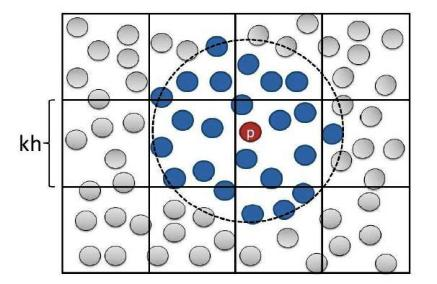
\includegraphics[scale=1]{figuras/grade.jpg}
	\caption{\textsc{Determinação das partículas vizinhas pelo método de Busca em Grades}}
	\vspace{-0.1cm}
	\legend{FONTE: \citeonline{Violeau}}
	\label{fig:grade}
\end{figure}
\begin{figure}[H]
	\centering
	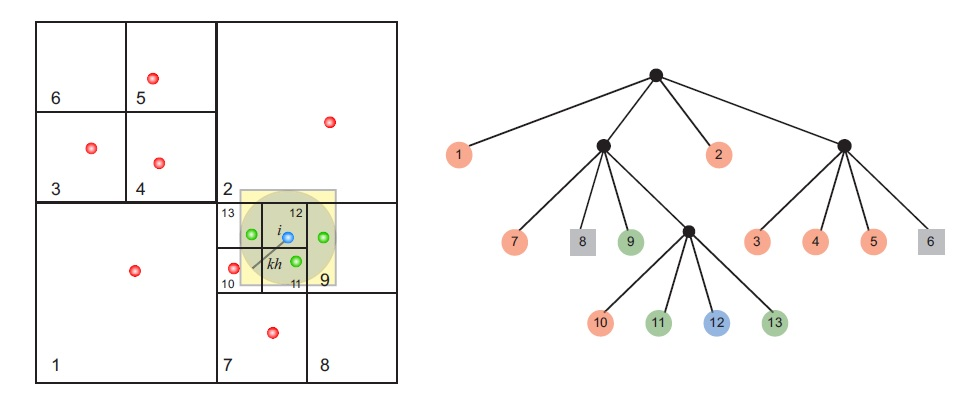
\includegraphics[scale=.8]{figuras/octree.jpg}
	\caption{\textsc{Determinação das partículas vizinhas usando Estruturas Adaptativas como as estruturas octree}}
	\vspace{-0.1cm}
	\legend{FONTE: \citeonline{Paiva2009}}
	\label{fig:octree}
\end{figure}

Para as condições de fronteira, existe a necessidade de manter o fluido, de certa forma, "confinado". Para tanto, há o método das Partículas Fantasmas, onde as fronteiras são partículas capazes de gerar forças de repulsão e de manter as demais partículas dentro do domínio desejado. Para tanto, as partículas são dispostas ao longo da fronteira com o intuito de repelir as partículas internas que se aproximam do contorno, conforme pode ser observado da Figura \ref{fig:particula_fantasma} que esquematiza este processo. No entanto, este tratamento pode ser difícil de ser mantido para geometrias mais complexas, conforme abordado no trabalho de \citeonline{Vacondio}.
\begin{figure}[H]
	\centering
	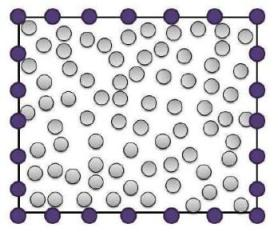
\includegraphics[scale=1]{figuras/particula_fantasma.jpg}
	\caption{\textsc{Tratamento das fronteiras usando Partículas Fantasmas}}
	\vspace{-0.1cm}
	\legend{FONTE: \citeonline{Queiroz}}
	\label{fig:particula_fantasma}
\end{figure} 

Para geometrias mais complexas, \citeonline{Paiva2007} propôs um método baseado na Reflexão Geométrica, Figura \ref{fig:colisao}, onde as partículas que irão colidir com a fronteira, partícula $t_0$, tem sua trajetória e velocidade corrigida, partícula $t_1$, como se realmente tivesse entrado em contato com a fronteira.
\begin{figure}[H]
	\centering
	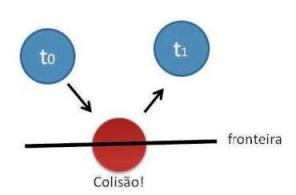
\includegraphics[scale=1]{figuras/colisao.jpg}
	\caption{\textsc{Tratamento das fronteiras usando Reflexão Geométrica}}
	\vspace{-0.1cm}
	\legend{FONTE: \citeonline{Queiroz}}
	\label{fig:colisao}
\end{figure}  

O assunto sobre o método SPH é amplo e seu uso tem evoluído nas mais diversas áreas do conhecimento e entretenimento, como bem destacado no trabalho de \citeonline{Paiva2009}. Junto com essa evolução estão os algoritmos que simulam as mais variadas geometrias e formas de escoamentos destacando-se, entre eles, o algoritmo proposto por \citeonline{Ramachandran2010}, intitulado PySPH, que será discutido no próximo capítulo.  


